\documentclass{article}
\usepackage[utf8]{inputenc}

% images
\usepackage{graphicx}
\graphicspath{ {./images/} }

% comments
\usepackage{comment}

% colored text
\usepackage[dvipsnames]{xcolor}

\title{Agents}
\author{Daniel Gigliotti}
\date{}

\begin{document}

\maketitle

\section{Rational agents}

\textbf{An agent} is an entity that perceives and acts, \textbf{everything that recognizes the environment through sensors and acts upon the environment through actuators}. \\


\textbf{A rational agent} (or intelligent agent), on the other hand, is a person or entity that \textbf{always aims to perform optimal actions} based on given premises and information. A rational agent can perform specific, predictable and repetitive tasks for applications with some level of individualism. \\


\textbf{How do an intelligent agent work?} Its main components are:
\begin{itemize}
\item \textbf{Sensors}: a device that detects environmental changes and sends the information to other devices;
\item \textbf{Actuators}: a device that convert energy into motion;
\item \textbf{Effectors}: a device that applies the motion to perform a specific task.
\end{itemize} 

\textbf{What is the difference between actuators and effectors?}
An actuator is a device that converts energy into motion, while an effector is a device that applies that motion to perform a specific task. For example, a motor is an actuator, while a robotic applies the motion generated by the motors to perform a specific task. \\

\textbf{Rationality} defines the level of being reasonable.

\newpage

\section{Agent and environment}

An AI system can be defined as the study of a rational agent and its environment. 
A rational agent can be anything that makes decisions, typically a person, robot or software. An agent can be seen as a black box interacting with the environment in two ways:

\begin{center}
    \begin{itemize}
        \item takes input from the environment (perceives)
        \item produces an output (acts)
    \end{itemize}
\end{center}

The agents sense the environment through sensors and act on their environment through actuators.

How can we implement this box? How do the system will convert perceptions into actions?

\section{Agent architecture}

Abstractly, an agent can be seen as a function that maps from percept histories to actions:

\begin{center}
    \begin{equation}
        f: P^{*} \rightarrow A
    \end{equation}
\end{center}

A $percept$ is a sequence of $perceptions$: maybe previous perceptions could help us in the future.

For a given task we seek the agent (or class of agents) with the best performance (which makes the action that maximizes the expected value of the performance measure given the percept sequence to date).
Computational limitations make perfect rationality unachievable.

\section{Problem solving}

Firstly we have the \textbf{problem formulation}: we define a set of states (called \textbf{state space}) and one among them as \textbf{initial state} (starting point).
Then we need to specify a \textbf{goal state} (or a set of goal states), that is the condition we want the agent to achieve. The agent will use artificial intelligence techniques such as search algorithms, decision making algorithms and machine learning to make decisions and take action to reach the goal state from the initial state; this step is called \textbf{search process}. 

The agent can implement the search process \textbf{online}, acting without complete knowledge (e.g. in real-time scenarios), or \textbf{offline}.

Online problem solving means that searching takes place as data becomes available, while in offline problem solving data is accumulated over a period of time and the model can search using all that information. 

\section{Agent types}

Five basic types of agents in order of increasing generality:

\begin{center}
    \begin{itemize}
        \item simple reflex agents
        \item model-based reflex agents
        \item goal-based agents
        \item utility-based agents
        \item learning agents
    \end{itemize}
\end{center}

\newpage

\section{Simple reflex agents}

\begin{center}
    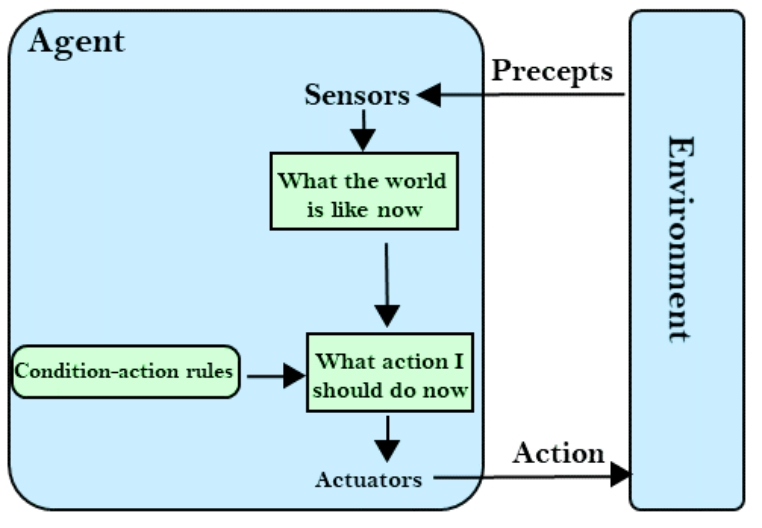
\includegraphics[scale=0.4]{images/simple_relfex_agent.jpg}
\end{center}

\textbf{TLDR: A simple reflex agent operates based on a condition-action rule. It selects actions solely based on the current percept (input) without considering the agent's history or future consequences.} \\

The current percept is used rather than the percept history to act by these agents. The core of these agents is the \textbf{condition-action rule set}. The condition-action rule set is a set of rules that map a condition to an action: they perceive something, they do something else in response to that. \\

Simple reflex agents are a direct connection between perception and action; they can't make prediction since the model does not know how the world will change in response to the action. They have very limited intelligence and require a fully observable environment. Environmental changes are not adaptable, meaning that if we want to act differently to a condition we need to change them (cause of the condition-action rule set). \\

\textcolor{ForestGreen}{
    \textbf{Example: Suppose the agent is a taxi that goes from point A to point B. This agent will have a set of condition-action rules like this:
    \begin{itemize}
        \item if car at crossroad 1: go left
        \item if car at crossroad 2: go right
        \item if traffic light is green: go forward
        \item ...
    \end{itemize}
    }
}

\newpage

\section{Model-based reflex agents}

\begin{center}
    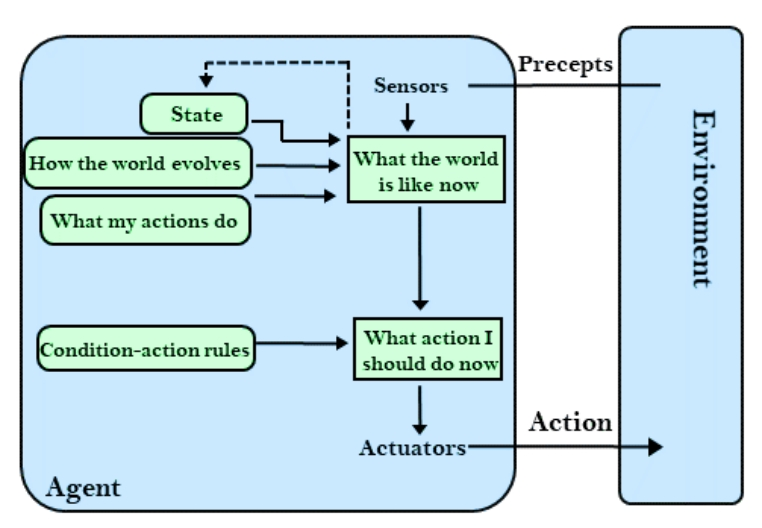
\includegraphics[scale=0.4]{images/model_based_reflex_agent.jpg}
\end{center}

\textbf{TLDR: A model-based agent maintains an internal model of the world, allowing it to keep track of the current state and predict the consequences of its actions.} \\

Model-based agents still have that sort of condition-action rule set and they don't have a goal. They have a model of the world; each time they take an action they know how that will effect the world; the action is still taken on the basis of the condition-action rule set. \\

\textbf{Basically we add a model of the world} to the agent to predict how the world will change based on its actions.

\begin{center}
    \begin{tabular}{p{0.45\textwidth}|p{0.45\textwidth}}
    
        Simple-reflex agents & Model-based agents \\
        
        \begin{itemize}
            \item look at the environment and act accordingly
        \end{itemize} & 
        \begin{itemize}
            \item look at the environment;
            \item ask themselves which effects will each action have;
            \item update the model;
            \item consult the same condition-action rule set;
            \item take the action;
        \end{itemize} 
    \end{tabular}
\end{center}

\newpage

\textcolor{ForestGreen}{\textbf{
    In the case of a model-based agent, the taxi agent maintains an internal model of the world, which includes relevant information about the environment, such as roads, traffic conditions, and any other pertinent details. This internal model allows the agent to have a representation of the current state of the world and predict the consequences of its actions.
    If we want the agent to go from A to B, it can identify multiple ways to do it but it does not know which is the best way: it knows that, if in point (a) it nees to turn right, if in point (b) it needs to go left and so on, but everything needs to be explicitly coded into the same condition-action rule set. This time the world is not static.
}}

\newpage

\section{Goal-based agents}

\begin{center}
    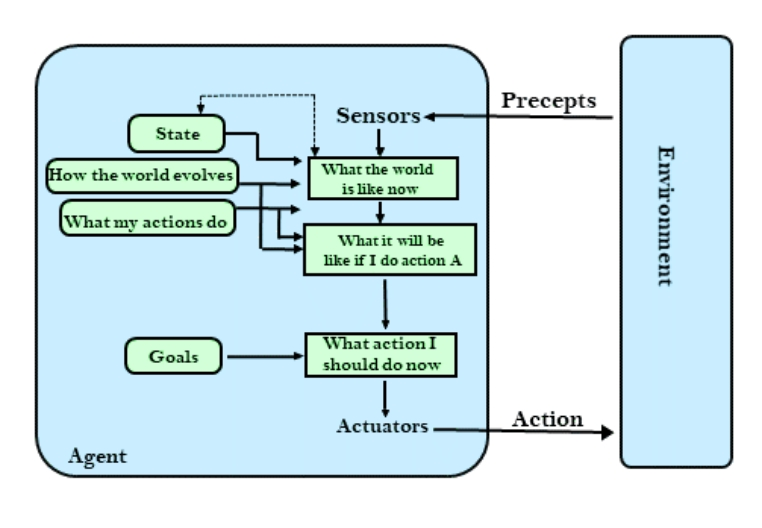
\includegraphics[scale=0.4]{images/goal_based_agent.jpg}
\end{center}

\textbf{TLDR: A goal-based agent selects actions based on its current state and a predefined goal. It uses its internal knowledge to identify the sequence of actions required to achieve the goal.} \\

Goal based agents use \textbf{goal information}. The main advantages are:

\begin{itemize}
    \item the knowledge supporting a decision is explicitly modeled and thereby modifications are allowed;
    \item the agent, knowing how the world evolve, can also project himself towards the future and say if a sequence of actions can eventually let him reach the goal;
\end{itemize}

These agents are more flexible because the knowledge that supports its decisions is represented explicitly and can therefore be easily modified. \\

\textcolor{ForestGreen}{\textbf{Referring to the previous example, a goal-based taxi agent easily adapt to reach a different point just by changing the goal from B to C (changing the destination of the taxi). The simple reflex/model-based reflex agent's rule set is difficult to adapt in comparison.}} 

\newpage

\section{Utility-based agents}

\begin{center}
    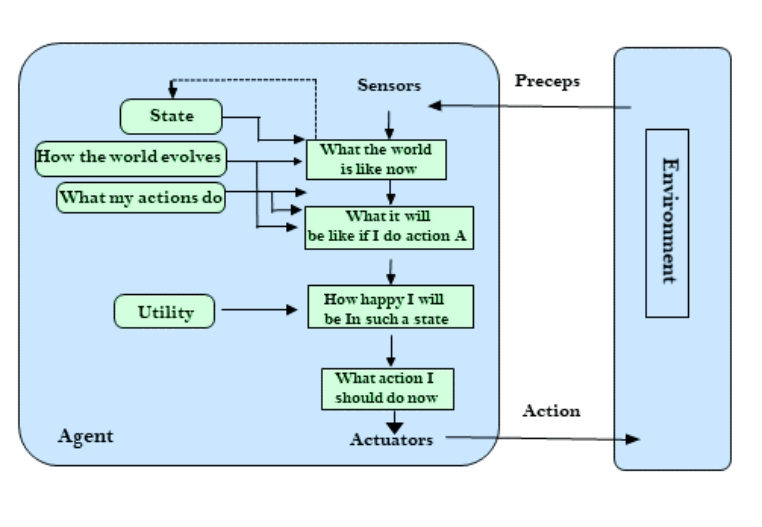
\includegraphics[scale=0.4]{images/utility_based_agent.jpg}
\end{center}

\textbf{TLDR: A utility-based agent makes decisions by assigning a utility value to each possible action. It considers both the immediate and long-term consequences of its actions to maximize overall utility.} \\

\textbf{Choices made by an utility based agent are based on utility}. The utility \textbf{measures the goodness of the outcome} of an action. The agent can therefore take \textbf{the best} action among the available options. \\

\begin{comment}
Using the aforementioned taxi examples, if the taxi is a goal-based agent, it can take one of many different paths to reach the goal and all of them are the same from its perspective. If the taxi is a utility-based agent, it will choose the best path according to a criterion (e.g. traffic conditions or shortness). \textbf{The goal alone is not enough to generate high quality behaviour in most environments}; many action sequences will get the taxi to its destination (thereby achieving the goal) but some are quicker, safer, more reliable or cheaper than others. \\
\end{comment}

\textcolor{ForestGreen}{\textbf{
    In the taxi domain, an utility-based taxi agent assigns a utility value to each potential path to the goal based on factors such as distance, traffic conditions etc. It can choose the path that maximizes this utility function.
}} \\

\textbf{Goal just provides a crude binary distinction between "happy" or "unhappy" states}. A performance measure assigns a score to any given sequence of environment states.

\newpage

Goals alone are not enough to generate high-quality behaviour in most environments. \\

\textcolor{ForestGreen}{\textbf{For example, many action sequences will get the taxi to its destination (thereby achieving the goal), but some are quicker, safer, more reliable or cheaper than others.}} \\

We have already seen that a performance measure assigns a score to any given sequence of environment states, so it can easily distinguish between more and less desirable ways of leading the agent to its goal. An agent’s utility function is essentially an internalization of the performance measure. Provided that the internal utility function and the external performance  measures  are  in  agreement,  an  agent  that  chooses  actions  to  maximize  its utility will be rational according to the external performance measure.

\vspace{2cm}

\begin{itemize}
    \item When there are conflicting goals, only some of which can be achieved  (for example, speed and safety), the utility function specifies the appropriate trade-off.
    \item When there are several goals that the agent can aim for, none of which can be achieved with certainty, utility provides a way in which the likelihood of success can be weighed against the importance of the goals.
\end{itemize}

An agent that possesses an explicit utility function can make rational decisions  with a general-purpose algorithm that does not depend on the specific utility function being maximized. 

\newpage

\section{Learning agents}

\begin{center}
    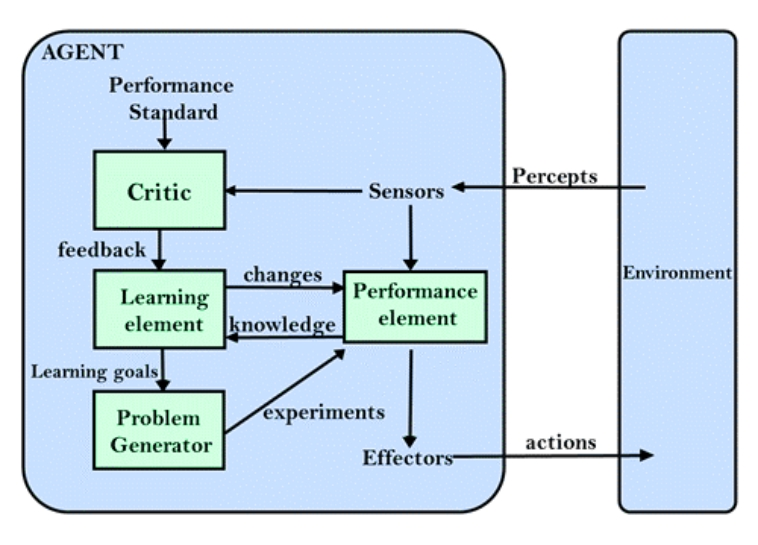
\includegraphics[scale=0.4]{images/learning_agent.jpg}
\end{center}

\textbf{TLDR: A learning agent improves its performance over time by learning from its interactions with the environment. It uses various techniques like supervised learning, reinforcement learning, or unsupervised learning to update its behavior.} \\

All the above agents can be turned into learning agents. A learning agent is an agent with the capability of learning from its previous experience. What is it needed to talk about learning agents?

\begin{itemize}
    \item $Learning\ element$: element that enables learning from previous experience;
    \item $Critic$: provides feedback on how well the agent is doing concerning a fixed performance standard;
    \item $Performance\ element$: the actions to be performed are selected;
    \item $Problem\ generator$: acts as a feedback agent that performs certain tasks such as making suggestions that will lead to new and informative experiences;
\end{itemize}

\end{document}
